\documentclass[11pt,a4paper]{article}
\usepackage[T1]{fontenc}
\usepackage[left=3cm, right=3cm, top=3cm, bottom=3cm]{geometry}
\usepackage{graphicx}
\usepackage{mathtools}
\usepackage{amssymb}
\usepackage{amsthm}
\usepackage{thmtools}
\usepackage{nameref}
\usepackage{hyperref}
\usepackage{times}
\begin{document}
\begin{center}
		\Large \textbf{{SUIT Dust Filtering Mechanism}}\\
	\normalsize Janmejoy Sarkar | 2024-06-30
\end{center}
	
	\section{Introduction}
	Spots introduced due to contaminants and dust grains is a common phenomenon on all optical and imaging systems. These patterns could be time dependent, wavelength dependent, parameter dependent- i.e. appearing only under certain observation configurations of the instrument, or a combination of the above factors. The nature of the dust spots could be like large blobs to small opaque spots. In the perview of  this document, we shall refer to a certain kind of contamination signature as `dust.' The contaminant spot should be smaller than or of the order of 25 pixels in size, and the counts within the spot should be comparable to the bias value of the image, the case being no data is recorded at the locations of `dust.' This algorithm automatically looks for such regions and replaces the `dust' with values interpolated from neighboring pixels by using morphological filters.
	
	\section{Methodology}
	\subsection{LED assisted Dust Mask Method}
	\begin{itemize}
		\item SUIT LED image is used to generate a mask of all dust particles.
		\item The large scale illumination pattern of the LED images is removed using multiscale structure isolation methods, similar to that used for generating PRNU profiles for SUIT CCD.
		\item A boxcar blurring with kernel size of 4 px is applied to remove single pixel scale non uniformities.
		\item Otsu thresholding is used to create a boolean mask of the dust spots. A morphological dilation filter is applied to this mask to increase the size of the regions representing the dust spots. This is done to ensure that the mask completely occupies the dust spot.
		\item Median filtering is applied on a copy of the Sun image, with a kernel size of 10 px. The kernel size is chosen such that dust spots the are completely replaced a median value of pixels from around the dust. A smaller kernel size shall reduce the size of the dust spot instead of completely eliminating it, while a large kernel size would lead to the loss of spatial information, while also being computationally more demanding.
		\item The mask is multiplied with the median filtered image, such that the result only contains information of the masked regions.
		\item The Sun image is multiplied with the inverse of the mask, such that the dust spot regions have no data.
		\item The two resultant images are added to have an image of the Sun where the dust spots have been replaced by the median of the neighbouring pixels.
		\begin{align*}
			Resultant~image = &[Sun~image * (1-Dust~Mask) ]\\
			&+ [Median~Filtered~Sun~Image * Dust~Mask]
		\end{align*}
		\item Figure \ref{fig:dustexample} shows an example of the dust filtering.
	\end{itemize}
	
		\begin{figure}
		\centering
		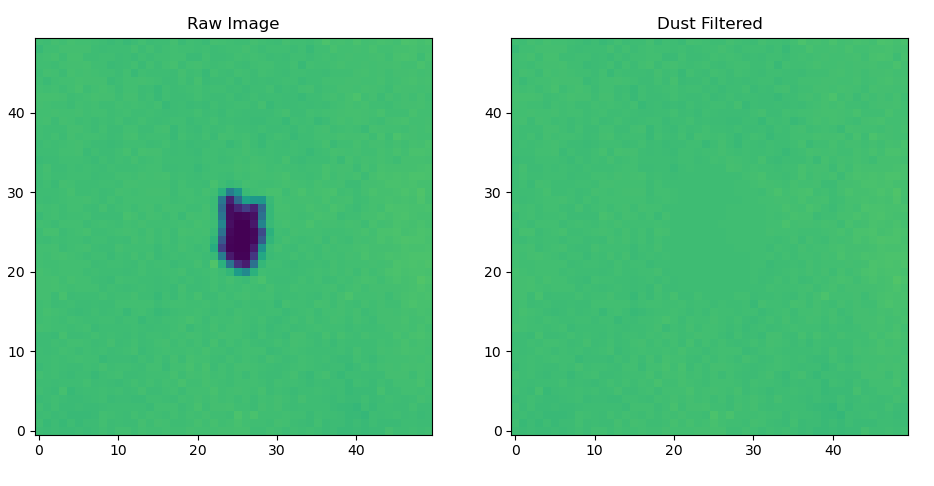
\includegraphics[width=0.7\linewidth]{pics/screenshot_2024-06-28_22-51-28.png}
		\caption{An example of a dust spot in an image, before and after applying dust correction.}
		\label{fig:dustexample}
	\end{figure}
	
	\subsection{Automated dust identification and removal method}

	\begin{itemize}
		\item An image is opened.
		\item A circular mask is generated using embeded Sun Center information. This helps to select the area of the Sun, excluding the background sky.
		\item The dust spots within the body of the Sun is identified based on a threshold. A binary image is generated with ones representing the regions of the dust spots. This image is dilated with a circular kernel of radius 6 pixels. The dilation helps to ensure that the dust spots in the generated dust mask is larger than the dust spot themselves.
		\item An erosion filter of 1 px radius is applied on a copy of the Sun image, followed by a dilation filter of radius 6 pixels. The prior erosion filter prevents the dilation of any scattered bright pixels, which might introduce artefacts. The dilation filter helps to fill the dust spots with values interpolated from the neighbouring pixels.
		\item The dust mask is multiplied with the filtered image, such that the result only contains information of the masked regions.
		\item The Sun image is multiplied with the inverse of the mask, such that the dust spot regions have no data.
		\item The two resultant images are added to have an image of the Sun where the dust spots have been replaced by the median of the neighbouring pixels. The results are represented in \ref{fig:screenshot2024-06-2822-50-31}.
		\begin{align*}
			Resultant~image = &[Sun~image * (1-Dust~Mask) ]\\
			&+ [Filtered~Sun~Image * Dust~Mask]
		\end{align*}
	\end{itemize}
	
		\begin{figure}
		\centering
		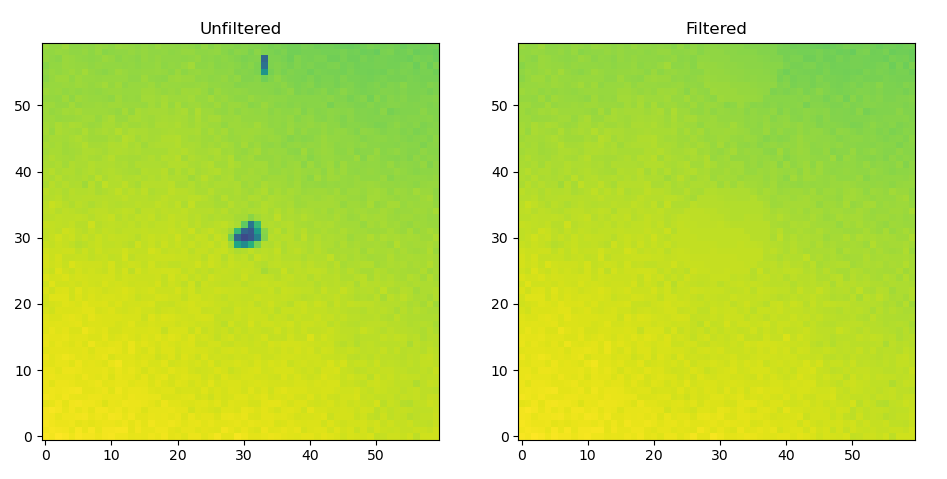
\includegraphics[width=0.7\linewidth]{pics/screenshot_2024-06-30_15-14-11.png}
		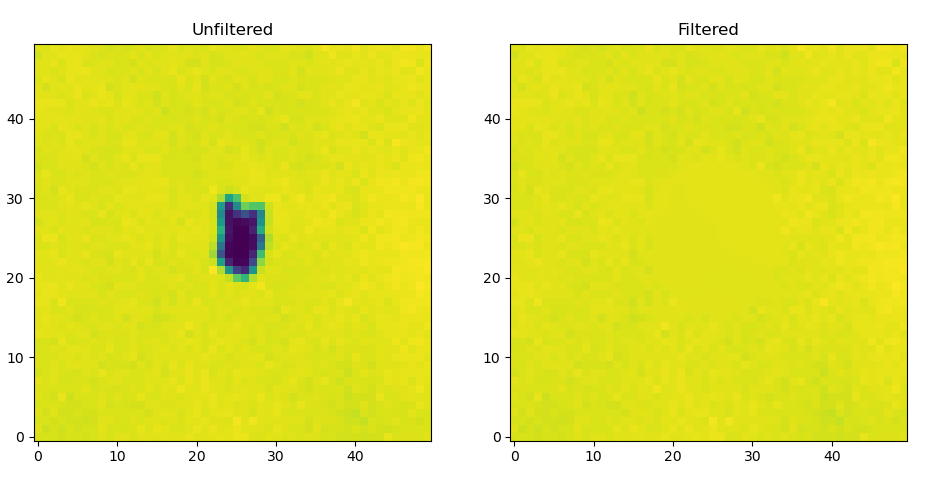
\includegraphics[width=0.7\linewidth]{pics/screenshot_2024-06-30_13-51-36.png}
		\caption{Example of the Automated Dust Identification and Removal Method, applied on an NB06 image of SUIT. Left and Right colums show the raw (Bias, Scatter and Flat corrected) and the filtered images respectively.}
		\label{fig:screenshot2024-06-2822-50-31}
	\end{figure}
	
	\section{Results and Conclusion}
	\subsection{LED Assisted Dust Mask Method}
	\begin{itemize}
		\item \textbf{Pros:} Effective in removing dust spots from the entire field of view.  It is effective in isolating dust structures and filtering them individually. 
		\item \textbf{Cons:} The dust pattern on the CCD may change with time. While the LED image closest to the image under usage is used, it is still not representative of the dust pattern at a given date. Therefore, there can be situations where some dust spots on an image of the Sun is not corrected as well as, some regions on the Sun could be over corrected
		\item \textbf{Future Scope:} While the LED based dust removal method might not be the best solution, it can be used to identify and remove contaminant patterns which do not appear opaque in the images. A multiscale filtering approach with LED images is under preparation.
	\end{itemize}
	
	\subsection{Automated dust identification and removal method}
	\begin{itemize}
	\item \textbf{Pros:} This method identifies dust spots based on thresholds. Therefore, it is more robust at identifying dust spots and filling them.
	\item \textbf{Cons:} It is dependent on thresholds, which might change based on the nature of throughput variation with time.
	\item \textbf{Future Scope:} An automated dynamic threshold setting method is being prepared to make the dust identification more robust. Updates will be reported in this document.
	\end{itemize}
	\begin{center}
		-x-
	\end{center}
\end{document}